\documentclass[a4paper]{article}
%\VignetteEngine{knitr::knitr}
%\VignetteIndexEntry{Estimation of the Number of Male Capercaillie on Leks of the French Pyrenees Mountains from 2010 to 2019}
%\VignetteDepends{knitr,ggplot2,dplyr,rjags,MCMCvis,rlang, purrr,tidyr,bayesplot, ade4, ggridges, gridExtra, coda}
\usepackage{fancyvrb}
\usepackage{color}
\usepackage{url}
\usepackage{amsfonts}
%\usepackage{pdfcolmk}
\usepackage{epsfig}
\usepackage[colorlinks=true,linkcolor=blue,urlcolor=blue,citecolor=blue]{hyperref}
\usepackage{longtable}
%\usepackage{natbib}
\usepackage{ucs}
\usepackage{savesym}
\savesymbol{iint}
\savesymbol{iiint}
\usepackage{amsmath}
\usepackage{rotating}
\usepackage{appendix}
%\usepackage[utf8]{inputenc}
\newlength{\defaultparindent}
\setlength{\defaultparindent}{\parindent}
\newenvironment{Default Paragraph Font}{}{}
\newcommand{\INT}[1]{\stackrel{\circ}{#1}}
\topmargin -1.5cm
\headheight 0.5cm
\headsep 1.0cm
\topskip 0.5cm
\textheight 24.5cm
\footskip 1.0cm
\oddsidemargin 0.0cm
\evensidemargin 0.0cm
\textwidth 16cm
\parskip 0.2cm
\parindent 1.0cm
\baselineskip 0.2cm



\title{ Estimation of the Number of Male Capercaillie on Leks of the
  French Pyrenees Mountains from 2010 to 2019 }
\author{Clement Calenge,\\
  Office Fran\c{c}ais de la Biodiversit\'{e}\\
  Saint Benoist -- 78610 Auffargis -- France.}
\date{June 2020}

\setlength{\parindent}{0cm}

%%%%%%%%%%%%%%%%%%%%%%%%%%%%%%%%%%%%%%%%%%%%%%%%%%%%%%%%%%%%%%%%%%%%%%%%%%%%%%
%%%%%%%%%%%%%%%%%%%%%%%%%%%%%%%%%%%%%%%%%%%%%%%%%%%%%%%%%%%%%%%%%%%%%%%%%%%%%%

\begin{document}

\maketitle
\tableofcontents




%%%%%%%%%%%%%%%%%%%%%%%%%%%%%%%%%%%%%%%%%%%%%%%%%%%%%%%%%%%%%%%%%%%%
%%%%%%%%%%%%%%%%%%%%%%%%%%%%%%%%%%%%%%%%%%%%%%%%%%%%%%%%%%%%%%%%%%%%
%%%%                                                            %%%%
%%%%                  The vignette starts here                  %%%%
%%%%                                                            %%%%
%%%%%%%%%%%%%%%%%%%%%%%%%%%%%%%%%%%%%%%%%%%%%%%%%%%%%%%%%%%%%%%%%%%%
%%%%%%%%%%%%%%%%%%%%%%%%%%%%%%%%%%%%%%%%%%%%%%%%%%%%%%%%%%%%%%%%%%%%

\newpage

\section*{Introduction}


This vignette is the supplementary material of the paper of Calenge et
al.The aim of this paper is to estimate the number of male
capercaillie in the 5 geographic regions of the French Pyrenees
mountains, for each period of two years between 2010 and 2019. A
companion package named \texttt{caperpyogm} contains the data and
functions used for this paper, and is required to reproduce the
calculations in this document. To install this package, first install
the package \texttt{devtools} and use the function
\texttt{install\_github} to install \texttt{caperpyogm}:

\begin{knitrout}
\definecolor{shadecolor}{rgb}{0.969, 0.969, 0.969}\color{fgcolor}\begin{kframe}
\begin{alltt}
\hlcom{## If devtools is not yet installed, type}
\hlkwd{install.packages}\hlstd{(}\hlstr{"devtools"}\hlstd{)}

\hlcom{## Install the package caperpyogm}
\hlstd{devtools}\hlopt{::}\hlkwd{install_github}\hlstd{(}\hlstr{"ClementCalenge/caperpyogm"}\hlstd{)}
\end{alltt}
\end{kframe}
\end{knitrout}

It is supposed throughout this vignette that the reader is familiar
with the model developed in this paper. Nevertheless, we will present
a brief reminder on this model in this vignette. This model combines
three datasets:\\

\begin{enumerate}
\item the results of counts of singing males carried out every period
  of two years on capercaillie leks, which allow to model the time
  changes in the mean abundance of on the various types of leks (KAL =
  known active leks; KIL = known leks with indeterminate activity
  status; UL = leks unknown at the time of the definition of the
  sampling design), and in the different geographic regions;\\

\item the results of the search for new, unknown leks in grid cells
  randomly selected in the whole area. This dataset was required to
  estimate the number of leks on our study area, which were unknown at
  the time of the definition of the sampling design.\\

\item the results of an experiment carried out to estimate the
  probability to detect an active lek unknown to the observer in a
  grid cell during a grid cell search. This experiment involved both
  experienced or inexperienced observers searching for leks unknown to
  them (but known to us).\\
\end{enumerate}

We developed two sub-models for (i) the mean number of males actually
present on a lek of a given type (KAL, KIL, UL), during a given period
and within a given geographic region, and (ii) the number of leks
unknown to us at the time of the definition of the sampling design in
a given geographic region.\\


In this document, we give a detailed information on this study, which
completes the information given in the paper:\\

\begin{itemize}
\item In section \ref{sec:notations-1}, we present all the
  mathematical notations used in the paper and in the appendix in a
  table.\\

\item In section \ref{sec:notat-model-descr}, we give a brief reminder
  on the structure of the model used to estimate the number of males,
  and we show how to use the datasets and functions given in the
  package to reproduce the calculations given in the paper. Note that
  all the functions included in this paper have a very detailed help
  page explaining how they should be used. This section contains
  additional elements not presented in the paper (residual analysis,
  analysis of the convergence and the mixing of MCMC chains,
  sensitivity to outliers, etc.).\\

\item In section \ref{sec:other-models-detect}, we demonstrate how a
  cross-validation approach was used to select the best model for the
  detection process during lek counts.\\

\item In section \ref{sec:lek--281}, we study more in detail the case
  of the lek \# 281. This lek is characterized by a strong residual in
  our model. We examined more precisely whether this lek had a strong
  influence on our inference.\\

\item In section \ref{sec:sens-our-model}, we considered in detail the
  criticisms of the N-mixture models by \cite{Barker2017} and
  \cite{Link2018}. In particular, we used simulations to assess the
  effect of unaccounted heterogeneity in detection probability as well
  as the effect of accidental double counting on the estimated number
  of males.\\
  
\item In section \ref{sec:history-program}, we give some additional
  elements describing the history of the monitoring program. In
  particular, we describe how the discovery that unknown leks were
  characterized by large number of males affected our program.\\
\end{itemize}



\section{Notations}
\label{sec:notations-1}

We present, in the table below, the notations used in this paper. We
distinguish several types of notations:\\

\begin{itemize}
\item D: data used to fit the model
\item P: stochastic parameter estimated with MCMC
\item N: other notations\\
\end{itemize}

In the table below, we give:\\

\begin{itemize}
\item the notation
\item the type of notation
\item a description of the variable or parameter\\
\end{itemize}


% latex table generated in R 4.1.0 by xtable 1.8-4 package
% Sun Feb 14 21:25:52 2021
\begin{tabular}{llp{12cm}}
  \hline
Notation & Type & Description \\ 
  \hline
$y_{i,t,k}$ & D & Number of detected males during count occasions $k$ of the year $t$ on lek $i$ \\ 
  $b(t)$ & N & Index of the two-year period containing the year $t$ \\ 
  $N_{i,b(t)}$ & P & Number of males actually present on lek $i$ during the two year-period $b(t)$ \\ 
  $p_{i,t,k}$ & P & Probability of detection of a male present on lek $i$ during count occasion $k$ of year $t$ \\ 
  $\alpha_d$ & P & Intercept of the model for the process of detection of males during counts \\ 
  $\beta_d$ & P & Slope of the number of observers in the model for the detection process of males during counts \\ 
  $o_{i,t,k}$ & D & Number of observers participating to the count occasion $k$ of the year $t$ on lek $i$ \\ 
  $e_{g(i),t}$ & P & Random effect of the year $t$ on the detectability of males in geographic region $g$ \\ 
  $\sigma_e$ & P & Standard deviation of the year random effect on the detectability of males during counts \\ 
  $\lambda_{i,b(t)}$ & P & Expectation of the Poisson distribution of the number of males on lek $i$ during period $b(t)$ \\ 
  $\kappa_{g(i),\ell(i),b(t)}$ & P & Parameter describing the average number of males during period $b(t)$ on a lek of type $\ell(i)$ in region $g(i)$ \\ 
  $\nu_{u(i)}$ & P & Random effect of the natural unit $u(i)$ \\ 
  $\eta_i$ & P & Random effect of the lek $i$ \\ 
  $\epsilon_{i,b(t)}$ & P & Overdispersion residual \\ 
  $\mu_{g(i),\ell(i)}$ & P & Mean of the average numbers of males during period $b(t)$ on leks of type $\ell(i)$ in region $g(i)$ \\ 
  $\sigma_{\kappa}$ & P & Standard deviation of the average numbers of males during period $b(t)$ on leks of type $\ell(i)$ in region $g(i)$ \\ 
  $\sigma_{\nu}$ & P & Standard deviation of the natural units random effects \\ 
  $\sigma_{\eta}$ & P & Standard deviation of the lek random effects \\ 
  $\sigma_{\epsilon}$ & P & Standard deviation of the overdispersion residuals \\ 
  $z_q$ & D & Whether the cell $q$ contains an unknown lek detected during a search of our program \\ 
  $f_q$ & D & Whether the cell $q$ was sampled in 2018--2019 \\ 
  $s_q$ & D & Whether the cell $q$ contains an unknown lek detected before the search of our program \\ 
  $b_q$ & P & Whether the cell $q$ actually contains an unknown lek \\ 
  $r_q$ & D & Proportion of the cell $q$ covered by the presence area of the capercaillie \\ 
  $h_q$ & D & Whether the cell $q$ already contains a known lek \\ 
  $\pi_q$ & P & Probability that the cell $q$ contains an unknown lek \\ 
  $a_{g(q)}$ & P & Intercept of the model predicting $\pi_q$ \\ 
  $b_{g(q)}$ & P & Slope of $r_q$ in the model predicting $\pi_q$ \\ 
  $d$ & P & Slope of $h_q$ in the model predicting $\pi_q$ \\ 
  $\beta$ & P & Probability of detection of an unknown lek during the search of a grid cell \\ 
  $\alpha$ & P & Probability that an unknown lek present in the cell was discovered prior to its sampling \\ 
  $S_c$ & D & Number of the known leks present in grid cell $c$ included in the search sector \\ 
  $D_c$ & D & Number of the known leks present in grid cell $c$ detected by the observer \\ 
  $N_c$ & D & Number of the known leks present in grid cell $c$ \\ 
  $\delta$ & P & Probability to detect a lek during a search when the lek is in the search sector \\ 
  $e(c)$ & N & Level of experience of the observers searching the cell $c$ \\ 
  $\zeta_{e(c)}$ & P & Probability that the search sector defines by the observer with experience $e(c)$ includes a lek present in a cell \\ 
  $S_{g\ell}$ & D/P & Number of leks of type $\ell$ in the region $g$ (to be estimated for UL \\ 
  $Q$ & D & Number of grid cells in the frame \\ 
  $n_{g\ell b}$ & P & Number of males on leks of type $\ell$ during the period $b$ in region $g$ \\ 
  $n_b$ & P & Number of males on all leks of the mountain range during period $b$ \\ 
   \hline
\end{tabular}





\section{Model description and model fit}
\label{sec:notat-model-descr}

We describe in this section the two sub-models required for the
estimation of the numbers of males present in the geographical regions
of the Pyrenees, for each two-years period between 2010 and 2019.

\subsection{Count model}
\label{sec:model-description}

\subsubsection{ Model description}
\label{sec:model-description-1}

We first describe the sub-model of the mean number of males detected
during the lek counts carried out in the French Pyrenees mountains
between 2010 and 2019.\\

Let $y_{i,t,k}$ be the number of males counted during the count
occasion $k$ of the year $t$ on the lek $i$. We model these counts
with a N-mixture model. We suppose that the number of detected animals
is the realization of a binomial distribution:
\begin{equation}
  \label{eq:eqy}
y_{i,t,k} \sim \mathcal{B}(N_{i,b(t)}, p_{i,t,k})
\end{equation}
where $N_{i,b(t)}$ is the number of males actually present on lek $i$
during the two-years period $b(t)$ including year $t$, and $p_{i,t,k}$
is the probability of detection characterizing this count occasion on
this lek, this year. We suppose the following detection model:
\begin{equation}
  \label{eq:detect}
\mbox{logit } p_{i,t,k} = \alpha_d + \beta_d \times o_{i,t,k} + e_{g(i),t}
\end{equation}

where $o_{i,t,k}$ is the number of observers present on lek $i$ during
count occasion $k$ of year $t$, $\alpha_d$ is the intercept of the
model, $\beta_d$ is the slope, and $e_{g(i),t}$ is a Gaussian random
effect characterizing year $t$ in the geographic region $g(i)$ where
the lek $i$ is located. More formally, we suppose:
$$
e_{g(i),t} \sim \mathcal{N}(0, \sigma_e)
$$
We discuss alternative detection models in section
\ref{sec:other-models-detect}.\\

Moreover, we suppose that the actual number of males $N_{i,b(t)}$ on
lek $i$ during the two-years period $b(t)$  containing the year $t$ is
the realization of a Poisson distribution:
\begin{equation}
  \label{eq:eqN}
  N_{i,b(t)}\sim \mathcal{P}(\lambda_{i,b(t)})
\end{equation}
And we suppose the following log-linear model for the expectation of
this distribution:
\begin{equation}
  \label{eq:eqlambda}
\log \lambda_{i,b(t)} = \kappa_{g(i),\ell(i),b(t)} + \nu_{u(i)}\times
I(\ell(i) =2) + \eta_i + \epsilon_{i,b(t)}
\end{equation}
Where $\kappa_{g(i),\ell(i),b(t)}$ is a random intercept
characterizing the type $\ell(i)$ of the lek $i$ (1 for KAL, 2 for
KIL, and 3 for UL) in the geographic region $g(i)$ containing lek $i$
during two-years period $b(t)$ including year $t$; $\nu_{u(i)}$ is a
random effect characterizing the effect of the natural unit $u(i)$
which contains the lek $i$ (note that a random effect characterizing
the natural unit is only included for KILs, see paper for an
explanation); $\eta_i$ is a random effect characterizing lek $i$, and
$\epsilon_{i,b(t)}$ is a Gaussian overdispersion residual.\\

We furthermore suppose the following distributions for these parameters:
\begin{eqnarray*}
\kappa_{g(i),\ell(i),b(t)} & \sim & \mathcal{N}(\mu_{g(i),\ell(i)},
  \sigma_{\kappa})\\
\nu_{u(i)} & \sim & \mathcal{N}(0,\sigma_\nu) \\ 
\eta_{i} & \sim & \mathcal{N}(0,\sigma_\eta^{\ell(i)})\\
\epsilon_{i,b(t)} & \sim & \mathcal{N}(0,\sigma_\epsilon)  
\end{eqnarray*}


\subsubsection{Fit of the count model}
\label{sec:fitmc}

We load the library \texttt{caperpyogm}, which contains the data and
the functions that we used to fit the model:


\begin{knitrout}
\definecolor{shadecolor}{rgb}{0.969, 0.969, 0.969}\color{fgcolor}\begin{kframe}
\begin{alltt}
\hlkwd{library}\hlstd{(caperpyogm)}
\end{alltt}


{\ttfamily\noindent\itshape\color{messagecolor}{\#\# Loading required package: ggplot2}}

{\ttfamily\noindent\itshape\color{messagecolor}{\#\# Loading required package: dplyr}}

{\ttfamily\noindent\itshape\color{messagecolor}{\#\# \\\#\# Attaching package: 'dplyr'}}

{\ttfamily\noindent\itshape\color{messagecolor}{\#\# The following objects are masked from 'package:stats':\\\#\# \\\#\#\ \ \ \  filter, lag}}

{\ttfamily\noindent\itshape\color{messagecolor}{\#\# The following objects are masked from 'package:base':\\\#\# \\\#\#\ \ \ \  intersect, setdiff, setequal, union}}

{\ttfamily\noindent\itshape\color{messagecolor}{\#\# Loading required package: rjags}}

{\ttfamily\noindent\itshape\color{messagecolor}{\#\# Loading required package: coda}}

{\ttfamily\noindent\itshape\color{messagecolor}{\#\# Linked to JAGS 4.2.0}}

{\ttfamily\noindent\itshape\color{messagecolor}{\#\# Loaded modules: basemod,bugs}}\end{kframe}
\end{knitrout}

All the datasets of the package are ``lazy-loaded'', i.e. they are
immediately available:

\begin{knitrout}
\definecolor{shadecolor}{rgb}{0.969, 0.969, 0.969}\color{fgcolor}\begin{kframe}
\begin{alltt}
\hlkwd{head}\hlstd{(lekcounts)}
\end{alltt}
\begin{verbatim}
##   lek period nbobs nbmales gr type natun year
## 1  81      1    -1       2  3    1     1    1
## 2 238      1     0       0  4    1     1    1
## 3 324      1     0       7  5    1     1    1
## 4 324      1     3      11  5    1     1    2
## 5   1      1     0       2  1    1     1    1
## 6   1      1     0       1  1    1     1    1
\end{verbatim}
\end{kframe}
\end{knitrout}

This data.frame contains the results of the counts carried out on all
leks in the Pyrenees mountains from 2010 to 2019. For each count
occasion, this data.frame contains:\\

\begin{itemize}
\item The lek label, numbered from 1 to 330
\item The two-years period during which  the count occurred
\item The number of observers. We have subtracted 2 to the number of
  observers, to improve the mixing of the MCMC chains.
\item The number of males counted on the lek
\item The number of geographic region containing the lek
\item The type of the lek (1 = KAL, 2 = KIL, 3 = UL)
\item The label of the natural unit containing the lek
\item The year during which the count occurred.\\
\end{itemize}

We have programmed the model in JAGS:

\begin{knitrout}
\definecolor{shadecolor}{rgb}{0.969, 0.969, 0.969}\color{fgcolor}\begin{kframe}
\begin{alltt}
\hlkwd{cat}\hlstd{(modelCountDetectBinREY)}
\end{alltt}
\begin{verbatim}
## model {
## 
##   ## Priors for top parameters of the state model
##   sigmanu~dgamma(0.01,0.01)
##   sigmaepsilon~dgamma(0.01,0.01)
##   sigmakappa~dgamma(0.01,0.01)
##   sigmaREY~dgamma(0.01,0.01)
## 
##   ## Priors for top parameters of the detection model
##   interceptpd~dnorm(0,0.1)
##   pente1pd~dnorm(0,0.1)
## 
## 
##   ## Priors for other parameters
##   for (i in 1:Ntypes) {
## 
##       sigmaeta[i]~dgamma(0.01,0.01)
## 
##       for (j in 1:Ngr) {
##          mukappa[j,i]~dnorm(0,0.1)
##          for (k in 1:Nperiods) {
##             kappa[j,i,k]~dnorm(mukappa[j,i], sigmakappa)
##          }
##       }
## 
##   }
## 
##   ## Random effect period
##   for (i in 1:Ngr) {
##     for (j in 1:Nyears) {
##         REY[i,j]~dnorm(0, sigmaREY)
##     }
##   }
## 
##   ## Random effects natural units
##   for (i in 1:Nnatun) {
##      nu[i]~dnorm(0,sigmanu)
##   }
## 
##   ## Expectation of the number of males
##   for (i in 1:Nleks) {
##       eta[i]~dnorm(0,sigmaeta[ellp[i]])
##       for (j in 1:Nperiods) {
##          epsilon[i,j]~dnorm(0,sigmaepsilon)
##          loglambda[i,j] <- kappa[gr[i],ellp[i],j]+nu[natun[i]]*ell2[i]+eta[i]+epsilon[i,j]
##          log(lambda[i,j]) <- loglambda[i,j]
##       }
##    }
## 
## 
## 
##   ## Likelihood
##   for (i in 1:Nlekperiods) {
##     N[i]~dpois(lambda[lek[i], period[i]]  )
##     for (k in 1:repetition[i]) {
##         logit(pd[i,k]) <- interceptpd + pente1pd*observers[i,k] + REY[gr[lek[i]],year[i,k]]
##         y[i,k]~dbin(pd[i,k], N[i])
##     }
##   }
## }
\end{verbatim}
\end{kframe}
\end{knitrout}


We now use the function \texttt{dataCount2jags} to prepare the data
to fit the JAGS model:


\begin{knitrout}
\definecolor{shadecolor}{rgb}{0.969, 0.969, 0.969}\color{fgcolor}\begin{kframe}
\begin{alltt}
\hlstd{dataList} \hlkwb{<-} \hlkwd{dataCount2jags}\hlstd{(lekcounts}\hlopt{$}\hlstd{lek, lekcounts}\hlopt{$}\hlstd{period,}
                           \hlstd{lekcounts}\hlopt{$}\hlstd{nbobs, lekcounts}\hlopt{$}\hlstd{nbmales,}
                           \hlstd{lekcounts}\hlopt{$}\hlstd{gr,} \hlkwd{as.numeric}\hlstd{(}\hlkwd{factor}\hlstd{(lekcounts}\hlopt{$}\hlstd{type)),}
                           \hlstd{lekcounts}\hlopt{$}\hlstd{natun, lekcounts}\hlopt{$}\hlstd{year)}
\end{alltt}
\end{kframe}
\end{knitrout}


We can now use the function \texttt{fitModelCount} to fit this
model. WARNING: THIS CALCULATION TAKES A VERY LONG TIME (several hours)
!!!! Note that we have included the results of this calculation as a
dataset of the package, so that the reader does not need to launch
this function to reproduce the other calculations:

\begin{knitrout}
\definecolor{shadecolor}{rgb}{0.969, 0.969, 0.969}\color{fgcolor}\begin{kframe}
\begin{alltt}
\hlstd{coefModelCountDetectBinREY} \hlkwb{<-} \hlkwd{fitModelCount}\hlstd{(dataList,} \hlstr{"modelCountDetectBinREY"}\hlstd{)}
\end{alltt}
\end{kframe}
\end{knitrout}



\subsubsection{MCMC chains mixing}
\label{sec:conv-model-fit}

Once the MCMC samples have been obtained, we can plot the chain for a
visual examination of the mixing. We present the traceplot for the
parameters $\kappa$ below:

\begin{knitrout}
\definecolor{shadecolor}{rgb}{0.969, 0.969, 0.969}\color{fgcolor}\begin{kframe}
\begin{alltt}
\hlkwd{library}\hlstd{(bayesplot)}
\end{alltt}


{\ttfamily\noindent\itshape\color{messagecolor}{\#\# This is bayesplot version 1.7.2}}

{\ttfamily\noindent\itshape\color{messagecolor}{\#\# - Online documentation and vignettes at mc-stan.org/bayesplot}}

{\ttfamily\noindent\itshape\color{messagecolor}{\#\# - bayesplot theme set to bayesplot::theme\_default()}}

{\ttfamily\noindent\itshape\color{messagecolor}{\#\#\ \ \ \ * Does \_not\_ affect other ggplot2 plots}}

{\ttfamily\noindent\itshape\color{messagecolor}{\#\#\ \ \ \ * See ?bayesplot\_theme\_set for details on theme setting}}\begin{alltt}
\hlkwd{library}\hlstd{(MCMCvis)}
\hlstd{cm} \hlkwb{<-} \hlkwd{MCMCchains}\hlstd{(coefModelCountDetectBinREY,}
                 \hlkwc{params}\hlstd{=}\hlkwd{c}\hlstd{(}\hlstr{"kappa"}\hlstd{,}\hlstr{"sigmakappa"}\hlstd{,}\hlstr{"sigmaepsilon"}\hlstd{,}\hlstr{"sigmaeta"}\hlstd{,}
                          \hlstr{"sigmanu"}\hlstd{,} \hlstr{"interceptpd"}\hlstd{,}\hlstr{"pente1pd"}\hlstd{,}\hlstr{"sigmaREY"}\hlstd{),}
                 \hlkwc{mcmc.list}\hlstd{=}\hlnum{TRUE}\hlstd{)}
\hlkwa{for} \hlstd{(i} \hlkwa{in} \hlnum{1}\hlopt{:}\hlkwd{length}\hlstd{(cm)) \{}
    \hlkwa{for} \hlstd{(j} \hlkwa{in} \hlkwd{c}\hlstd{(}\hlstr{"sigmakappa"}\hlstd{,}\hlstr{"sigmaepsilon"}\hlstd{,}\hlstr{"sigmaeta[1]"}\hlstd{,}
                \hlstr{"sigmaeta[2]"}\hlstd{,}\hlstr{"sigmaeta[3]"}\hlstd{,}\hlstr{"sigmanu"}\hlstd{,}\hlstr{"sigmaREY"}\hlstd{))}
        \hlstd{cm[[i]][,j]} \hlkwb{<-} \hlnum{1}\hlopt{/}\hlstd{cm[[i]][,j]}
\hlstd{\}}
\hlkwd{mcmc_trace}\hlstd{(cm,} \hlkwc{regex_pars}\hlstd{=}\hlstr{"kappa"}\hlstd{)}
\end{alltt}
\end{kframe}

{\centering 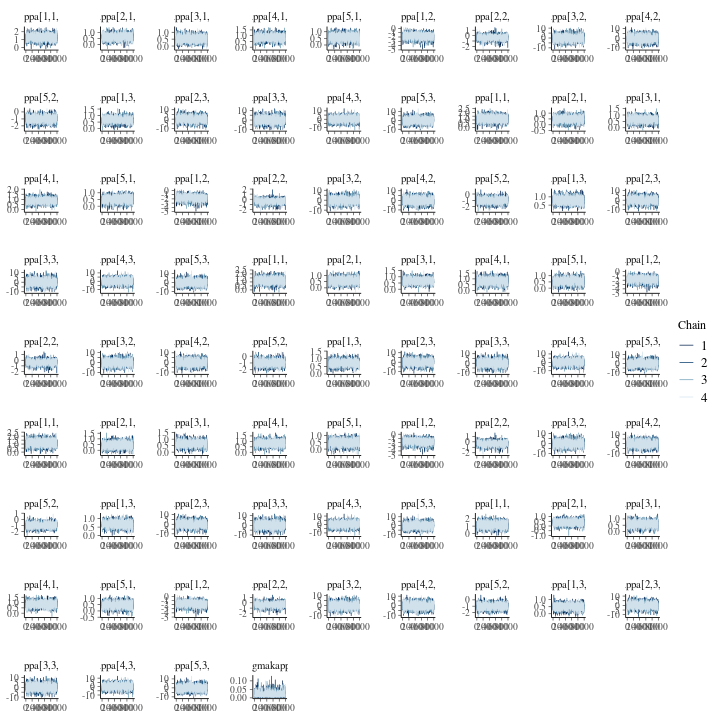
\includegraphics[width=\linewidth,height=\linewidth]{caperpy-traceplot-kappa-1} 

}



\end{knitrout}

We also present the traceplot for the variances of the state model:

\begin{knitrout}
\definecolor{shadecolor}{rgb}{0.969, 0.969, 0.969}\color{fgcolor}\begin{kframe}
\begin{alltt}
\hlkwd{mcmc_trace}\hlstd{(cm,} \hlkwc{regex_pars}\hlstd{=}\hlkwd{c}\hlstd{(}\hlstr{"sigmakappa"}\hlstd{,}\hlstr{"sigmaepsilon"}\hlstd{,}\hlstr{"sigmaeta"}\hlstd{,}
                            \hlstr{"sigmanu"}\hlstd{))}
\end{alltt}
\end{kframe}

{\centering 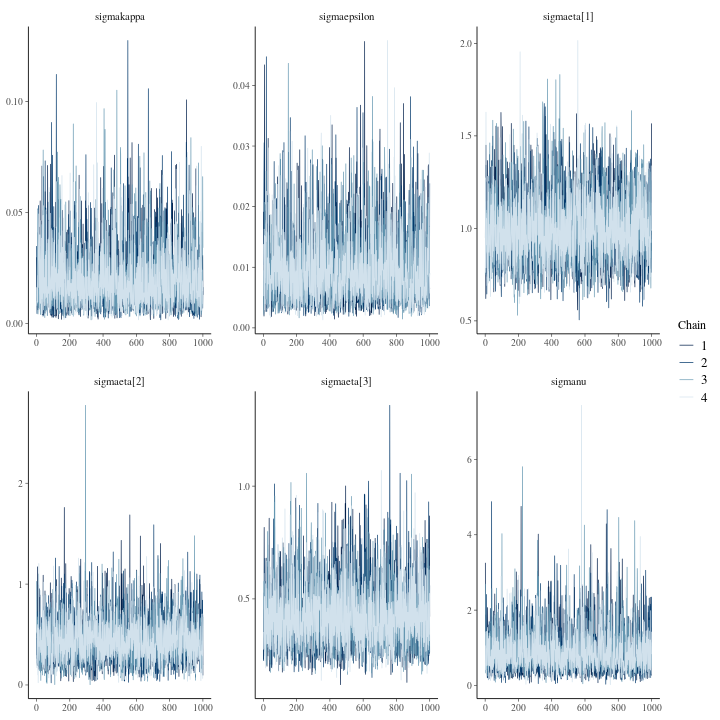
\includegraphics[width=\linewidth,height=\linewidth]{caperpy-traceplot-sigma-1} 

}



\end{knitrout}

Finally, we present the parameters for the detection model:

\begin{knitrout}
\definecolor{shadecolor}{rgb}{0.969, 0.969, 0.969}\color{fgcolor}\begin{kframe}
\begin{alltt}
\hlkwd{mcmc_trace}\hlstd{(coefModelCountDetectBinREY,}
           \hlkwc{regex_pars}\hlstd{=}\hlkwd{c}\hlstd{(}\hlstr{"REY"}\hlstd{,}\hlstr{"interceptpd"}\hlstd{,}\hlstr{"pente1pd"}\hlstd{,}\hlstr{"sigmaREY"}\hlstd{))}
\end{alltt}
\end{kframe}

{\centering 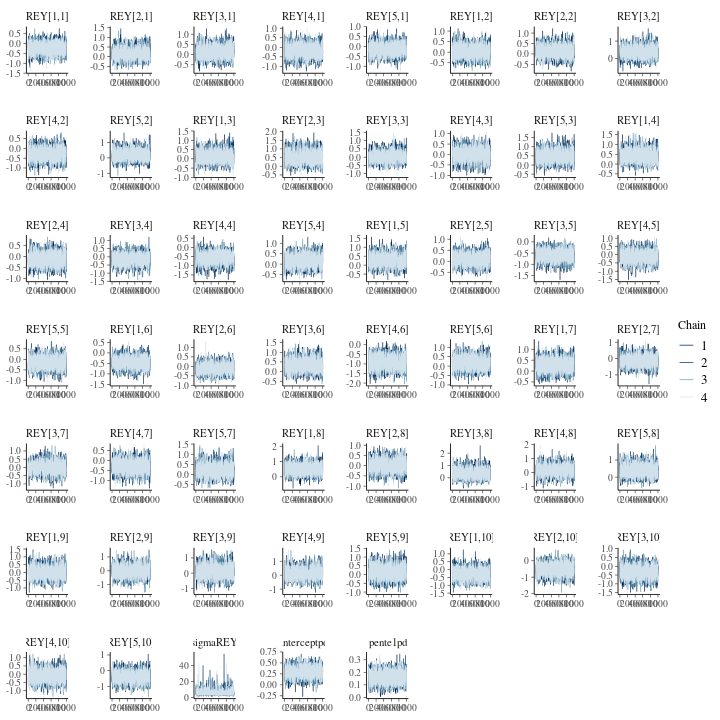
\includegraphics[width=\linewidth,height=\linewidth]{caperpy-traceplot-detection-1} 

}



\end{knitrout}

We also calculate the Gelman diagnostic for the parameters. To save
some space, we do not show the results of this diagnostic in this
vignette and leave it to the reader to check the correct mixing based
on this diagnostic:

\begin{knitrout}
\definecolor{shadecolor}{rgb}{0.969, 0.969, 0.969}\color{fgcolor}\begin{kframe}
\begin{alltt}
\hlkwd{gelman.diag}\hlstd{(cm)}
\end{alltt}
\end{kframe}
\end{knitrout}

\subsubsection{Identifiability of the parameters}
\label{sec:ident-param}






















































































































